\documentclass[12pt,a4paper,oneside]{article}
\usepackage[pdftex]{graphicx}
\usepackage{layout} 
\usepackage{caption}
\usepackage{booktabs}

% Theorem
%\usepackage{amsthm}

\usepackage[english]{babel}
%\usepackage[ngerman]{babel}


% Querformat

%\usepackage{pdfscape}


% Falls overfull hboxen entstehen, rechts markieren
%\overfullrule=1mm

%Abkürtzbgen

\usepackage{acronym}

\usepackage{harvard}
\usepackage{adjustbox}
\usepackage{lscape}
\usepackage[list=true]{subcaption}

%
% Tabellen
%
\usepackage{array}
\usepackage{tabularx}
\usepackage{ifthen}
\usepackage{amsfonts}
\usepackage{booktabs}
\usepackage{siunitx}
\usepackage{caption}

% python highlithing

\usepackage{minted}


% Einrückung von Aufzählungen
\usepackage{enumitem}


\usepackage{pgfplots}
%
%
\usepackage{lmodern}
\usepackage[doublespacing]{setspace}
%\usepackage{microtype}
\usepackage{adjustbox}
\usepackage{amsmath}
\usepackage{amssymb}
\usepackage{placeins}
%
% Textpositionierung
%
\usepackage{pstricks}
%
% Umlaute
%
\usepackage[utf8]{inputenc}
%\usepackage[T1]{fontenc}


%\usepackage[options]{nohyperref} 
\usepackage{url}

% footer header

\usepackage{fancyhdr}

\usepackage[hang, flushmargin]{footmisc}
%\usepackage[all]{nowidow}
%\captionsetup[table]{aboveskip=0pt}
%\captionsetup[table]{belowskip=0pt}
\setlength{\textfloatsep}{0.1cm}
%\graphicspath{ {C:\Users\David\Dropbox\Bachelorarbeit\Plots} }
%\clubpenalty=10000
%\widowpenalty=10000 
%\displaywidowpenalty=10000
\setlength{\parskip}{3ex plus 2ex minus 2ex}
%\usepackage{cite}
%\usepackage[round]{natbib}


\newcommand{\HRule}{\rule{\linewidth}{0.5mm}}
\singlespacing
\makeatletter
\newcommand{\miniscule}{\@setfontsize\miniscule{4.8}{4.8}}%
\newcommand{\midiscule}{\@setfontsize\midiscule{8.1}{8.1}}%

%%%%%%%%%%%%%%%%%%%%%%%%%%%%%%%%%%%%%%%%%%%%%%
% Umgegungen für Hypothesen
%%%%%%%%%%%%%%%%%%%%%%%%%%%%%%%%%%%%%%%%%%%%%
\newcounter{chyp}
\newenvironment{Hypothese}%
{
\singlespacing
  %\par
  \flushleft
  \stepcounter{chyp}\textbf{Hypothese
  \Roman{chyp}}:
  %\par\smallskip
}

\newcounter{csubhyp}
\newenvironment{Subhypothese}%
% { 

%   %\par
%   \singlespacing
  
%   \flushleft
%   \textit{\stepcounter{csubhyp}\textbf{Unterhypothese 
%     \Roman{chyp}.\alph{csubhyp}}:
%   %\par
%   }
% }



%\begin{Hypothese}
%    Die Anzahl der Beiträge ist ungleichmäßig auf die Nutzer verteilt.
%\end{Hypothese}
  
%\begin{Subhypothese}
%Die Gesamtlänge der Beiträge ist ungleichmäßig auf die Benutzer verteilt.
%\end{Subhypothese}


%%%%%%%%%%%%%%%%%%%%%%%%%%%%%%%%%%%%%%%%%%%%%
% Ende Hypotehsen Umgebung
%%%%%%%%%%%%%%%%%%%%%%%%%%%%%%%%%%%%%%%%%%%%%


%%%%%%%%%%%%%%%%%%%%%%%%%%%%%%%%%%%%%%%%%%%%%
% Begin Theoreme Umgebung
%%%%%%%%%%%%%%%%%%%%%%%%%%%%%%%%%%%%%%%%%%%%%


\newtheorem{defi}{Definition}
\newtheorem{satz}{Satz}
\newtheorem{bsp}{Beispiel}
%%%%%%%%%%%%%%%%%%%%%%%%%%%%%%%%%%%%%%%%%%%%%
% Ende Theoreme Umgebung
%%%%%%%%%%%%%%%%%%%%%%%%%%%%%%%%%%%%%%%%%%%%%

%\pagestyle{myheadings}
%\hypersetup{
%    pdfborder = {0 0 0}
%}

\begin{document}

%%%%%%%%%%%%%%%%%%%%%%%%%%%%%%%%%%%%%%%%%%
% Hilfe: ftp://ftp.tex.ac.uk/tex-archive/macros/latex/contrib/fancyhdr/fancyhdr.pdf
% Kopfzeile formatieren
\fancyfoot{}
\pagestyle{fancy}
%\fancyhead[C]{\leftmark}
\fancyhead[R]{\thepage}
%\rhead{\thesectionname}
%\rfoot{\thepage}
%%%%%%%%%%%%%%%%%%%%%%%%%%%%%%%%%%%%%%%%%%

 
 
 
 \selectlanguage{ngerman}
\setlength{\textheight}{240mm}
\setlength{\textwidth}{150mm}
%\setlength{\voffset}{0.46cm}
\setlength{\hoffset}{2cm}
%\setlength{\marginparsep}{0cm}
%\setlength{\marginparwidth}{0cm}
\setlength{\headsep}{1cm}
\setlength{\oddsidemargin}{0cm}
\setlength{\headheight}{0cm}
\setlength{\topmargin}{0cm}
\setlength{\footskip}{8pt}
\begin{titlepage}
	\begin{center}
	\textsc{\LARGE Zeppelin Universität}\\[1.5cm]
	\textsc{\Large zwischen Wirtschaft, Kultur und Politik}\\[0.5cm]

	% Title
	\singlespacing
	\HRule \\[0.4cm]
	{ \huge \bfseries Arbitrage zwischen digitalen Gütermärkten %The Limits of Multi-Market Arbitrage
	\\[0.4cm] }
%	{ \huge \bfseries Diversität in anonymen Online-Diskussionen \\[0.4cm] }

	\HRule \\[1.5cm]
	\end{center}
	
\begin{flushleft} \large

\emph{Autor, Matrikelnummer:}\\

%
% Jeder trägt noch seinen Namen ein
%
Christopher Helm, 13201294\\
\singlespacing
\emph{Studiengang:}\\
Corporate Management and Economics\\
Zeppelin University, Friedrichshafen
\singlespacing
\emph{Betreuer:}\\
Prof. Dr. Marcel Tyrell\\*
Institute of Entrepreneurship \& Finance, Zeppelin University, Friedrichshafen, Germany

\newline

%Professor für Unternehmer- und Finanzwissenschaften\\
%Institutsleiter und Fachbereichssprecher Corporate Management & %Economics\\
Dr. Tim Alexander Herberger\\*
Department of Finance, Bamberg University, Bamberg, Germany\\
\singlespacing

%\emph{Abgabetermin:}\\
 %\newcommand{\todayIV}{\leadingzero{\day}.\leadingzero{\month}.\the\year} , 
% \today, 
%Spring Term
%\end{flushleft}
%\end{titlepage}

% oben links vorerst keine Überschrifen wiederholen
\fancyhead[L]{}
\fancyhead[R]{}
%\newpage
%\doublespacing
%\pagenumbering{roman}
%\emph{EINFÜHRUNGSZITAT}
%\rput(13cm,5cm){Schreibe mit Blut: und du wirst erfahren, dass Blut Geist ist.}
%\rput(16.2cm,5cm){Friedrich Nietzsche, 1883}

%\newpage
%\renewcommand{\abstractname}{\section*{Abstract}}
%\abstractname{}
%Diese Ausarbeitung 


\renewcommand*\listfigurename{Abbildungsverzeichnis}
\renewcommand*\listtablename{Tabellenverzeichnis}
\renewcommand{\contentsname}{Inhaltsverzeichnis}
\renewcommand{\refname}{Quellen}
\newpage   

\fancyhead[R]{\thepage}
\pagenumbering{roman}
\tableofcontents


\newpage

%Abbildungsverzeichnis
\listoffigures % Abbildungsverzeichnis
\newpage
%Tabellenverzeichnis
\listoftables % Tabellenverzeichnis
\newpage
%\phantomsection \addcontentsline{toc}{section}{Abkürzungsverzeichnis}

\section*{Abkürzungsverzeichnis}
\begin{acronym}[Bash]
 \acro{CMC}{Computer-mediated-Communication}
 \acro{FTF}{Face-to-Face-Communication}
 \acro{SIDE}{Social Identitydeindividuation Theory}
 % immer \ac{abkürzung hier}
\end{acronym}
\newpage
\fancyhead[L]{\rightmark}
\pagenumbering{arabic}


%%%%%%%%%%%%%%%%%%%%%%%%%%%%%%%%%%%%%%%%%%%%%%%%%%%%%%%%%%%%%%%%%%%%%%%%%%%%%%%%%%%%%%%%%%%%%%%%%%
%%%%%%%%%%%%%%%%%%%%%%%%%%%%%%%%%%%%%%%%%%%%%%%%%%%%%%%%%%%%%%%%%%%%%%%%%%%%%%%%%%%%%%%%%%%%%%%%%%
%                    Hier beginnt die Latex Einführung
%%%%%%%%%%%%%%%%%%%%%%%%%%%%%%%%%%%%%%%%%%%%%%%%%%%%%%%%%%%%%%%%%%%%%%%%%%%%%%%%%%%%%%%%%%%%%%%%%%
%%%%%%%%%%%%%%%%%%%%%%%%%%%%%%%%%%%%%%%%%%%%%%%%%%%%%%%%%%%%%%%%%%%%%%%%%%%%%%%%%%%%%%%%%%%%%%%%%%
\onehalfspacing


 \selectlanguage{ngerman}
 
 
% \section{Latex Einführung}
% \subsection{Dies ist die Unterüberschrift}
% \subsubsection{Dies ist die Unter-Unterüberschrift}
% Normaler Text kann ohne besonderes Wissen eingefügt werden. Einen erzwungenen Zeilenumbruch
% generiert man durch wie man sieht. Aufzählungen macht man mit folgendem
% \textit{Konstrukt}: 

% \begin{description}
%   \item[Nummerierte Aufzählung]~\par
%   \begin{enumerate}
%       \item Weitere Aufzählung
%       \begin{enumerate}
%          \item erstens.
%          \item zweitens.
%       \end{enumerate}
%       \item Toter Punkt
%   \end{enumerate}
   
   
%   \item[Nichtnummerierte Aufzählung]~\par
%   \begin{itemize}
%       \item Unteraufzählung
%       \begin{itemize}
%          \item erstens.
%          \item zweitens.
%       \end{itemize}
%       \item der andere Punkt.
%   \end{itemize}
% \end{description}

% Durch den Befehl \textit{newpage} erzwingt man einen Seitenbumbruch. 

% \subsection{Tabellen}
% Tabellen sind schwieriger zu schreiben:

% %%%%%% Beginn von der Tabelle
% \begin{singlespace}
% \captionof{table}{Tabellenbeschriftung}
% \noindent\begin{tabularx}{.90\textwidth}{|l|c|r|X|} %140mm astatt \textwidth
%     % Das X steht oben für die Spalte, die automatisch and die Seitenbreite angepasst werden soll!!
   
    
    
%     \hline
%     \textbf{1 Zeile fett} & \textbf{2 Zeile fett}  & \textbf{3 Zeile fett} & 4 Spalte \\ \hline \hline
%     Monday & 11C & 22C & A clear day with lots of sunshine.  
%     However, the strong breeze will bring down the temperatures. \\ \hline
%     Tuesday & 9C & 19C & Cloudy with rain, across many northern regions. Clear spells
%     across most of Scotland and Northern Ireland,
%     but rain reaching the far northwest. \\ \hline
%     \end{tabularx}

% \end{singlespace}
% %%%%% Ende der Tabelle    




% Danach sollte es mit Text weitergehen \footnote{footnote text} bevor die nächste Überschfrift kommt.Danach sollte es mit Text weitergehen bevor die nächste Überschfrift kommt.Danach sollte es mit Text weitergehen bevor die nächste Überschfrift kommt.Danach sollte es mit Text weitergehen bevor die nächste Überschfrift kommt.Danach sollte es mit Text weitergehen bevor die nächste Überschfrift kommt.Danach sollte es mit Text weitergehen bevor die nächste Überschfrift kommt.Danach sollte es mit Text weitergehen bevor die nächste Überschfrift kommt.

% \subsection{Zitate}
% So sieht ein Zitat aus: I always thought something was fundamentally wrong with the universe  
% \cite[P. 16]{Adams1995} und das nächste Zitat \cite[P. 2000]{Helm2012} und das nächste einmal mit zwei Autoren \cite[P. 16]{ShariShariandHansGlueck:2010}

% \subsection{Bilder}
% So wird ein Bild eingefügt: 
% \begin{figure}[h!]
% %\centering
% 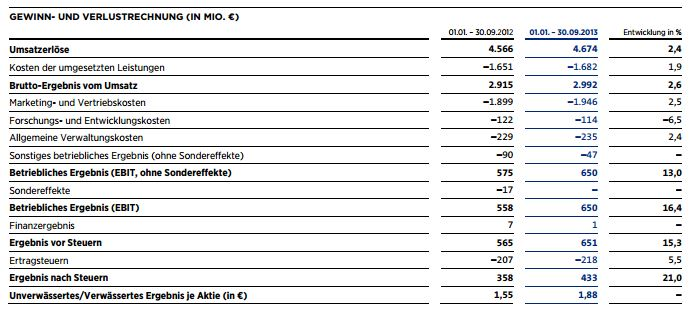
\includegraphics[width=.90\textwidth]{Beiersdorf2013Q3.JPG}
% \caption{Gewinn- und Verlustrechnung: Beiersdorf}
% \label{fig:univerise}
% \end{figure}

% Danach sollte es mit Text weitergehen \footnote{footnote text} bevor die nächste Überschfrift kommt.Danach sollte es mit Text weitergehen bevor die nächste Überschfrift kommt.Danach sollte es mit Text weitergehen bevor die nächste Überschfrift kommt.Danach sollte es mit Text weitergehen bevor die nächste Überschfrift kommt.Danach sollte es mit Text weitergehen bevor die nächste Überschfrift kommt.Danach sollte es mit Text weitergehen bevor die nächste Überschfrift kommt.Danach sollte es mit Text weitergehen bevor die nächste Überschfrift kommt.

% \begin{figure}[h!]
% %\centering
% 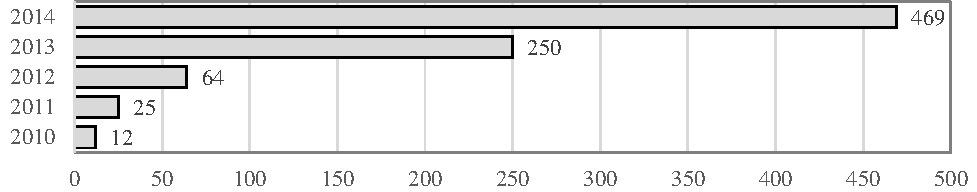
\includegraphics[width=.90\textwidth]{crawl-Zeit1-sicherhheit_cropped.pdf}
% \caption{Gewinn- und Verlustrechnung: Beiersdorf}
% \label{fig:univerise}
% \end{figure}

% Danach sollte es mit Text weitergehen \footnote{footnote text} bevor die nächste Überschfrift kommt.Danach sollte es mit Text weitergehen bevor die nächste Überschfrift kommt.Danach sollte es mit Text weitergehen bevor die nächste Überschfrift kommt.Danach sollte es mit Text weitergehen bevor die nächste Überschfrift kommt.Danach sollte es mit Text weitergehen bevor die nächste Überschfrift kommt.Danach sollte es mit Text weitergehen bevor die nächste Überschfrift kommt.Danach sollte es mit Text weitergehen bevor die nächste Überschfrift kommt.




%%%%%%%%%%%%%%%%%%%%%%%%%%%%%%%%%%%%%%%%%%%%%%%%%%%%%%%%%%%%%%%%%%%%%%%%%%%%%%%%%%%%%%%%%%%%%%%%%%
%%%%%%%%%%%%%%%%%%%%%%%%%%%%%%%%%%%%%%%%%%%%%%%%%%%%%%%%%%%%%%%%%%%%%%%%%%%%%%%%%%%%%%%%%%%%%%%%%%
%                    Hier beginnt das echte Dokument!!!
%%%%%%%%%%%%%%%%%%%%%%%%%%%%%%%%%%%%%%%%%%%%%%%%%%%%%%%%%%%%%%%%%%%%%%%%%%%%%%%%%%%%%%%%%%%%%%%%%%
%%%%%%%%%%%%%%%%%%%%%%%%%%%%%%%%%%%%%%%%%%%%%%%%%%%%%%%%%%%%%%%%%%%%%%%%%%%%%%%%%%%%%%%%%%%%%%%%%%



\newpage

\section{Einleitung}
\textit{Warum sollen Meinungen falsch sein? Letztlich sind die wissenschaftlichen Thesen auch nur Meinungen, obgleich solche, bei denen unter ihresgleichen ein Konsens besteht. Das macht aber die Aussagen nicht besser oder wahrer. Wenn Theorien oder Thesen widerlegt werden, sind sie es auch nicht, es herrscht nur ein Konsens vor, dass sie es seien. Also sind Massenmeinungen zu wissenschaftlichen Aussagen lediglich ein demokratischer Ausgleich von Gegenmeinungen, für die in der genannten Masse auch wiederum ein Konsens besteht!} \cite{eemueller}

Dieser Leserkommentar zu einem Artikel der Zeitung ZEIT ONLINE stellt die wissenschaftliche These der kollektiven Meinung gleich. Auch wenn über die logischen Schlüsse in diesem Kommentar diskutiert werden kann: Der Anspruch, dass private Meinungen von bekannten oder auch nicht bekannten Personen die Realität zunehmend stärker beeinflussen, zeigen verschiedene Beispiele in der Vergangenheit: Ein gehackter Twitter Account führt zu einem kurzzeitigen Kursrückgang an der Wallstreet \cite{njacobsen}. Unternehmen erhalten im Rahmen ihrer Social Media Aktivitäten Rück\-mel\-dungen der Kunden und reagieren auf unterschiedliche Art und Weise \cite{rmueller}. Pressemeldungen werden mehrmals täglich publiziert und können direkt kommentiert werden, ohne dass eine zeitliche Verzögerung durch den Druck der Zeitung entsteht. Solch reaktive Beteiligung kann darüber hinaus zu negativen Wellen der Meinungsäußerungen im Netz führen \cite{hofmann2013krise}. Die Diskussionen in dem neuen öffentlichen Raum (Internet) haben somit nicht nur Auswirkungen auf die virtuelle, sondern auch auf die reale Welt.

Dieses digitale Potential haben verschiedene Firmen bereits erkannt. Sie ermöglichen Personen, die bisher noch nicht im Kontakt mit der Firma stehen einen bedingten Zugang zu der eigenen Entwicklungs- und Forschungsabteilung \cite{enkel2014applying}. Dies soll den Firmen zusätzliche innovative Flexibilität ermöglichen \cite{gassmann2006open}. Die Öffnung der Unternehmen hat zur Folge, dass die normalen Angestelltenverhältnisse in Frage gestellt werden. So kann es sein, dass es neben den bezahlten Mitarbeitern eines Unternehmens freiwillige und zum Teil bezahlte, nicht physisch anwesende Helfer gibt, die ihre Erfahrungen und Ideen aus eigenem Interesse teilen \cite{stachbert}. Diese digitale Zusammenarbeit bzw. Diskussion wird in der Literatur \ac{CMC} genannt und unterscheidet sich von der Zusammenarbeit bei dem die Gruppenmitglieder physisch anwesend sind (\ac{FTF}).

Das Diversity Management muss auf diese Veränderung reagieren. Von verschiedenen Autoren wurde bereits untersucht, ob erkennbare und nicht direkt erkennbare Attribute von Individuen in Arbeitsgruppen einen Einfluss auf den Erfolg der Gruppe haben \cite{ivancevich2000diversity,ely2001cultural,van2004work,beinrauch2012diversity,vashanti2012}. Die Beobachtung, dass die Heterogenität der Gruppenteilnehmer den Erfolg der Gruppe beeinflussen, kann auch in der digitalen Zusammenarbeit festgestellt werden \cite{bargh2002can}. Es liegen bereits Untersuchungen vor, die die Heterogenisierung des Personals eines Unternehmens als Vorbereitung auf die heterogenen Konsumenten und Abnehmer unterstützen \cite{vashanti2012}. Die Frage, wie Unternehmen die neuen freiwilligen Helfer analysieren können, um deren Interaktion zu komponieren, ist gegenwärtig noch unbeantwortet \cite{oiestad201454,Rothmann201466,Mangematin20141}.

\newpage
\section{Theorie}
\subsection{Online-Märkte}
Die Erforschung der Diversität ist ebenso divers wie Ihre Einheiten der Analyse \cite[S. 1200]{harrison2007s}. Da bereits verschiedene Einordnungen der bestehenden Literatur versucht wurden, soll diese theoretische Betrachtung eine erweiterte Diversitäts-Definition erarbeiten \cite{jackson2003recent,ashkanasy2002diversity}. Durch diese gezielte Betrachtung werden drei Kernfaktoren isoliert und der dazugehörige Stand der Forschung detailliert dargestellt. 

Zuerst soll das Verständnis von Diversität in dieser Arbeit durch eine erweiterte Definition systematisiert werden. Dabei wurde folgende Definition als Grundlage verwendet: \textit{"Die Verteilung der persönlichen Attribute auf interdependente Mitglieder einer Arbeitsgruppe"} \cite[S. 802]{jackson2003recent}. Es wurde bereits erkannt, dass die Teilnehmer einer Arbeitsgruppe durch die Diversität im beruflichen als auch im nicht-beruflichen Umfeld geprägt werden \cite{van2004work,vashanti2012}. Aus diesem Grund wurde die zuvor genannte Definition erweitert, um bisher unbeachtete Einflüsse durch Personen, die nicht im direkten Zusammenhang mit dem Unternehmen stehen, aufzunehmen.

\begin{defi}[Diversität]
Der Begriff Diversität bezieht sich auf die Ver\-teil\-ung von persönlichen Attributen auf inter\-dependente Personen einer Gruppe.
\end{defi}

Diese Erweiterung ist notwendig, um auch in allen sozialen Interaktionen Diversitätsforschung betreiben zu können. Die reduzierte Betrachtung von Diversität auf den Unternehmenskontext verkennt oft die Komplexität des Diversitätsmanagements. Der Grad an Diversität in Unternehmen scheint vollständig durch das Unternehmen selbst kontrollierbar aufgefasst zu werden \cite{varela2010sinn}. Durch diese Erweiterung der Definition soll die Interdependenz der beruflichen und nicht-beruflichen Diversität der Mitarbeiter aufgenommen werden, sofern dies die Organisation beeinflusst. Die allgemeine in einer Gesellschaft beobachtbare Akzeptanz von Unterschiedlichkeiten soll dabei nicht diskutiert werden \cite{king}.

Im nächsten Schritt soll der Umgang des Unternehmens mit der Analyse, Beeinflussung und Kontrolle von Diversität definiert werden. Das durch Unternehmen angewendete Management der Diversität umfasst dabei alle freiwilligen Aktionen, die die Offenheit der Firmenkultur erweitert und die Individualität jedes Menschen akzeptiert (\cite[S. 773]{triandis1994workplace} kombiniert mit \cite[S. 159]{kirton2009costs}). Hierbei soll darauf hingewiesen werden, dass die Begriffe kulturelle Diversität, Diversität, Multikulturalismus und Diversität einer Arbeitsgruppe in der Literatur häufig als Synonyme verwendet werden \cite{ewoh2013}. Aus diesem Grund wird in dieser Ausarbeitung Diversität von dem Management der Diversität ausdrücklich unterschieden. Eine zu der oben genannten Definition ähnliche Beschreibung von Diversitätsmanagement soll an dieser Stelle für die weitere Bearbeitung festgehalten werden.

\begin{defi}[Diversitäts Management]
A voluntary organizational program designed to create greater inclusion of all individuals into informal social networks and formal company programs \cite[S. 61]{gilbert1999dm}.
\end{defi}


% \begin{satz}
% Unterschiede entstehen in dem Vergleich von Individuen untereinander. Individuen können sowohl in der beruflichen als auch in der nicht-beruflichen Welt gewollt oder auch ungewollt von einander abhängig sein.  
% \end{satz}
% Schon in der frühen Diversitätsliteratur kann erkannt werden, dass die Diskriminierung von Menschen anderer Hautfarbe ein missbrauchtes Unterscheidungskriterium war, dass sowohl den Alltag als auch den beruflichen Werdegang aller Beteiligten prägte \colorbox{yellow}{Quelle}.
% \begin{bsp}
% "Dieser Schein enthielt das Versprechen, dass allen Menschen - ja, schwarzen Menschen ebenso wie weißen - die unveräußerlichen Rechte auf Leben, Freiheit und den Anspruch Glück garantiert würden." \cite{king}
% \end{bsp}

Diese Definitionen ermöglichen nun eine strukturierte Betrachtung von drei für diese Ausarbeitung wichtigen Herausforderungen der Forschung. Diese drei Herausforderungen werden hier im Hinblick auf die folgende Fallstudie ausführlich dargestellt. Dies ermöglicht später das Ergebnis der Fallstudie in der Literatur einzuordnen und zu bewerten.

\textit{1. Faktor:} In der Literatur wird Diversität häufig in erkennbare und nicht direkt erkennbare (intellektuelle) Diversität kategorisiert \cite{harrison1998beyond,lapid1998diversity}. Ein Großteil der Untersuchungen entscheiden sich für Attribute der Persönlichkeit, die äußerlich erkennbar oder zumindest bei einer Befragung der Person durch eine sich ausschließende Ja-Nein-Frage feststellbar sind. Somit zählt auch die sexuelle Orientierung zu den sogenannten erkennbaren Attributen oder der primären Dimension von Diversität \cite{lapid1998diversity}. Die Erforschung der primären Dimension ist weit verbreitet. So beschäftigten sich von 63 Einzelarbeiten 89\% der Arbeiten mit von außen erkennbaren Attributen \cite[S. 804]{jackson2003recent}.

\textit{2. Faktor:} Ein möglicher Schritt zur Analyse von Diversität ist die multidimensionale Betrachtung von Diversität. Diese von der Theorie geforderte Herangehensweise soll bisher unabhängig analysierte Variablen im Verbund betrachten. Durch die Erhöhung der Kontrollvariablen wird einer Verzerrung von ausgelassenen Variablen vorgebeugt. Dabei erhöht die theoretisch geprägte Forderung die Menge der zu erhebenden Daten \cite{jackson2004diversity,joshi2009role}. So ist es durchaus möglich, dass über 8.000 Teams befragt werden, um in 39 Studien unterschiedliche Kontexte anzutreffen. Auf diese Weise war es möglich, den Einfluss von Diversität zu messen und Einflüsse durch verschiedene Kontexte zu kontrollieren \cite{joshi2009role}. In vielen Untersuchungen ist nicht eindeutig, welche Variablen zur Kontrolle des Kontextes genutzt werden müssen, um einer Messverzerrung durch ausgelassene Variablen vorzubeugen. Diese Schwierigkeit besteht durch die offene Definition des Kontexts, in dem die Diversität gemessen wird \cite[S. 812]{jackson2003recent}. 

\textit{3. Faktor:} Neben der Einführung von Kontrollvariablen auf die Ausprägung von Diversität, wird die Operationalisierung von Diversität noch offen diskutiert. Ebenen der Diversität werden häufig auf Basis der Zugäng\-lich\-keit von Informationen gebildet \cite{harrison1998beyond}. Bei dieser Herangehensweise besteht die Möglichkeit weitere Ebenen der Zugänglichkeit hinzuzufügen \cite{lapid1998diversity}. Ein relativ junges Verfahren operationalisiert Diversität nach dem Inhalt der Informationen und bewertet diese auf Grundlage des Informationsträgers \cite{harrison2007s}. So wird sowohl die hierarchische Ebene, die Haltung und der Bildungs\-Hintergrund zur Beurteilung der Diversität einer Gruppe verwendet. Dabei ist zu beachten, dass bei der zuletzt genannten Operationalisierung die einzelnen Variablen separat evaluiert werden \cite{harrison2007s}. Bei den zuvor genannten Verfahren wird häufig angenommen, dass sich die gemessenen Ebenen gegenseitig beeinflussen oder sogar gegenseitig erklären können \cite{lawrence1997perspective,harrison1998beyond,lapid1998diversity}.


\subsection{Digitiale Risikopräferenz}
Nicht alle Studien können einen signifikanten Einfluss des Kontexts auf die Wirkung der Diversität auffinden \cite[S. 693]{jackson2004diversity}. Es ist jedoch bekannt, dass der Kontext des Internets einen Einfluss auf die Äu\-ße\-rungen und Aktionen der Nutzer hat. Die Interaktion von \ac{FTF} unterscheidet sich dabei stark von jeglicher \ac{CMC} \cite{kiesler1984social,siegel1986group,lea1992paralanguage,walther1996computer}. Der Kontext der CMC wurde in zahlreichen Studien mit der FTF verglichen. Dabei stellte sich heraus, dass Leistungen oder Beiträge der Personen gleichmäßiger auf die Gruppe verteilt sind \cite{siegel1986group,mcguire1987group}. Außerdem bearbeiten CMC-Gruppen Aufgaben unter Zeitrestriktionen besser, sofern die Aufgaben wenig soziale und emotionale Interaktion erfordern \cite{gallupe1991unblocking,straus1994does}. Gleichzeitig steigt das Volumen von ungehemmten Äußerungen \cite{kiesler1984social,siegel1986group}.\footnote{Der Kontext der Fallstudie wurde somit zur besseren Analyse vollständig auf \ac{CMC} beschränkt \cite{dey2001understanding}.}

\begin{defi}[Kontext]
Context is any information that can be used to characterize the 
situation of an entity. An entity is a person, place, or object that is 
considered relevant to the interaction between a user and an 
application, including the user and applications themselves. \cite[S. 5]{dey2001understanding}
\end{defi}

% Exakte Bestimmung des Kontexts bedeutet in dem vorliegenden Fall, dass die fünf am häufigsten verwendeten Analysen für den Kontext (Aufgabenstellung, Kultur des Unternehmens, Stimmung in der Gruppe, strategischer Kontext und die Dauer der Zusammenarbeit) in dem Untersuchten Material nicht existieren.

Der Kontext der CMC ist ausführlich in der Literatur beschrieben. Grund\-sätzlich wurde die Frage diskutiert, ob die Persönlichkeit  im \ac{CMC} Kontext identisch mit der im \ac{FTF} Kontext beobachteten Persönlichkeit ist \cite{walther1996computer}. Solche Annahmen gehen so weit, dass die Persönlichkeit, die in einem \ac{FTF} erkannt wird, sich vollständig von der Persönlichkeit unterscheidet soll, die während einer \ac{CMC} beobachtet wird \cite{lea1992paralanguage}. Diese Teilung der Persönlichkeits\-beschreibung wurde auch mit \textit{\ac{SIDE}} beschrieben \cite{lea1992flaming}. Diese Deindividualisierung wird wie folgt begründet: Interagierende Personen in einem \ac{CMC} Kontext müssen auf Basis weniger Informationen ein Bild des Kommunikationspartners erstellen. Diverse \ac{FTF} Informationen (z. B. Gesichtszüge) sind bei der reinen Kommunikation per Text daher unzugänglich. Eine Person versucht daher auf einer reduzierten Datenbasis ein vollständiges Persönlichkeitsbild zu erstellen \cite{joinson2001self}.

Neben dieser Trennung von Persönlichkeiten in einem \ac{CMC} und \ac{FTF} Kontext vertreten verschiedene Forscher eine pragmatische Auffassung von Beschreibungen der Persönlichkeiten. Diese Forschung versucht nicht die Persön\-lich\-keit in dem Kontext zu erkennen. Die Beschreibung der Persönlichkeit wird auf die Beschreibung der Rolle einer Person in einem Kontext reduziert \cite{bargh2002can,geller1994rolle}. 
%Die Anwendung von Rollen zur Beschreibung von Personen ist in der Sozialforschung üblich. 
Viele der verwendeten Definitionen beziehen sich jedoch häufige auf die wie folgt definierte soziale Rolle \cite[S. 252]{schaefer1992grund}. 

\begin{defi}[Soziale Rolle]
Ein Bündel normativer Verhaltenserwartungen, die von einer Bezugsgruppe oder mehreren Bezugsgruppen an Inhaber bestimmter sozialer Positionen herangetragen werden. 
% R.n sorgen für regelmäßiges, vorhersagbares Verhalten als Voraussetzung für kontinuierlich planbare Interaktionen und erfüllen somit eine allgemeine soziale Orientierungsfunktion. Die Verhaltenserwartungen werden zwar an Individuen herangetragen, beziehen sich aber auf die sozialen Positionen, die die Individuen einnehmen, sind also auf Individuen als Positionsträger gerichtet.
\end{defi}

Diese Art der Beschreibung erlaubt es einen Teil der Person vollständig zu beschreiben, ohne die vollständige Person mit dieser Beschreibung abdecken zu wollen \cite{suler1999get}. Durch die Verwendung von Rollen kann die Beschreibung einer Person auf Basis der in der CMC erhaltenen Daten erfolgen, ohne dass die Beschreibung an Reliabilität verliert, da sie nicht die Persönlichkeit zu erklären versucht. Die Rollen werden individuell und unabhängig von einander beobachtet. So können selbst im \ac{CMC} Kontext verschiedene Rollen von einer Person erkannt werden. Ob diese Rollen aggregiert werden können, kann am Ende der Beobachtung überprüft werden, falls eine vollständige Beschreibung der Persönlichkeit generiert werden soll \cite{suler2004online}. Eine Wertung der verschiedenen Rollen kann nach der Aggregation vorgenommen werden \cite{rogers1951client,higgins1987self}. Diese durch das Internet hinzugewonnene Analyseebene der CMC stellt somit eine besondere Möglichkeit der Individuen dar, Rollen einzunehmen \cite{turkle2011life}.

Die soziale Rolle unterscheidet sich somit stark von der analysierten Rolle der Person in einem \ac{CMC} Kontext. Das Verständnis der \ac{CMC} Rolle wurde zur weiteren Analyse in eine Definition überführt \cite[S. 34]{rogers1951client,higgins1987self,bargh2002can}. Da anonyme Internetnutzer keine Bezugsgruppe haben, die sie kennen, kann die Definition der Sozialen Rolle nicht übernommen werden. Falls Internetnutzer häufig im \ac{CMC} Kontext interagieren, kann zusätzlich zu der CMC Rolle eine Soziale Rolle erkannt werden, da die ehemalig anonymen Nutzer durch ihre Aktivität eine Bezugsgruppe finden.\footnote{Diese Reindividualisierung wurde in der Fallstudie nicht weiter untersucht, da das Nutzerverhalten über verschiedene Zeitungsartikel hinweg keine Interaktionsmuster einzelner Nutzer erkennen lies.}

\begin{defi}[\ac{CMC} Rolle]
Von außen erkennbare Facette einer Person in dem untersuchten Kontext.
\end{defi}






%\subsection{Hypothesenbildung}
% Die umfassende theoretische Analyse ermöglicht es nun für den \ac{CMC} Kontext Hypothesen zu formulieren, die die explorative Analyse von Diversität ermöglicht. 

Auf Basis der zuvor genannten Theorie können folgende Hypothesen formuliert werden:
\begin{Hypothese}
    Die Anzahl der Beiträge ist gleichmäßig auf die Nutzer verteilt.
\end{Hypothese}
\begin{Hypothese}
    Das Thema der Diskussion hat einen erkennbaren Einfluss auf die Anzahl und Länge der Beiträge.
\end{Hypothese}
\begin{Hypothese}
    Die Beiträge der Teilnehmer stehen in Zusammenhang mit dem Inhalt der Artikel.
\end{Hypothese}

Diese Hypothesen ermöglichen eine gezielte Analyse der Fallstudie. Der bereits durch Literatur beschriebene Kontext konnte bereits definiert werden. Dadurch können mögliche Widersprüche, die sich im Bezug auf die bestehende Literatur ergeben, erkannt werden. So kann festgestellt werden: Personen, die die Diskussion lediglich lesen, können nicht beobachtet werden. Somit ist die Diversität der \ac{CMC} bedingt durch den aktiv erbrachten Beitrag. Die genannten Hypothesen gelten somit nur für aktive Teilnehmer. 

%#######################################################################################
\newpage
\section{Daten}
Diese explorative Studie soll einen Einblick in die Kommunikation von freiwillig interagierenden Online-Kunden auf der Plattform des Unternehmens ZEIT ONLINE bieten. Die Untersuchung ermöglicht es bisher unbe\-schriebene Interaktionen von Kunden in einem festgelegten Kontext zu beobachten.

Die Beschreibung der Kunden in Form von Rollen ermöglicht es die verwendeten quantitativen Methoden anzuwenden. Durch den Verweis auf Rollen eines Internetnutzers in einem einheitlichen Kontext, kann eine quantitative Textanalyse angesetzt werden. Der Kontext wurde aus methodischen Gründen so gewählt, dass die Internetnutzer lediglich eine Möglichkeit der Interaktion haben (öffentliche Kommentarfunktion). Es müssen demnach keine zusätzlichen Kontrollvariablen für verschiedene Kontexte verwendet werden. Die Stichprobe wurde hinsichtlich Wochentag, Tageszeit und Themenbereich der Interaktion auf Homogenität überprüft.

Um durch eine Triangulation von Datentypen die Reliabilität und Validität der vorerst quantitativ belegten Aussagen zu ermöglichen, wurde die Aussage in den vermerkten Fällen durch eine qualitative Textanalyse  wiederholt über\-prüft \cite{eisenhardt1989building,yin2009case}. Von diesem Verfahren wurde verstärkt bei der Analyse der einzelnen Kommentare Gebrauch gemacht.

\subsection{Erhebung}
Die Wahl der Online-Zeitung ZEIT ONLINE als Forschungskontext basiert auf zwei Gründen, die eine statistische Analyse ermöglichen sollen. Die Über\-prüfung auf Kontrollvariablen, die im Theorieteil als mögliche Einflussfaktoren besprochen wurden, waren dabei das vorgelagerte Kriterium des Auswahlprozesses.

Es wurde die Interaktionshäufigkeit von verschiedenen Online-\-Platt\-for\-men überprüft. Um eine große Stichprobe analysieren zu können, kamen grundsätzlich alle Plattformen in Frage, die über eine öffentliche Kommentar- bzw. Interaktionsfunktion verfügen. Diese öffentliche Kommentarfunktion ist für soziale Netzwerke nicht gegeben. Um ein hohes Kommentarvolumen vorfinden zu können, wurden verschiedene Online Bereiche von deutschen Zeitungen analysiert (Die Tageszeitung, ZEIT ONLINE, Frankfurter Allgemeine Zeitung, Handelsblatt, Süddeutsche Zeitung, Welt am Sonntag).

Nachdem Online-Zeitungen als Forschungskontext festgelegt waren, fiel auf, dass manche Zeitungen die Kommentare zensieren. Dabei zensieren manche Zeitungen den Kommentar durch bloßes Löschen. Andere Zeitungen wie ZEIT ONLINE kürzen den Kommentar um problematische Passagen und kennzeichnen den Eingriff der Redaktion. Um zu gewährleisten, dass die Kommentare einheitlich bereinigt sind, mussten Daten einer Plattform verwendet werden. Durch die Verwendung von ZEIT ONLINE ist erstens gewährleistet, dass eine Zensur nachweisbar ist. Zweitens wird angenommen, dass die Zensur der Kommentare an einheitlichen Kriterien von den Mitarbeitern von ZEIT ONLINE vorgenommen wurde. Diese Annahme wurde überprüft, indem Kommentaren gesucht und gefunden wurden, die ZEIT ONLINE oder die Autoren kritisieren.

\subsection{Aggregation und Verknüpfung}

\begin{figure}[h!]
%\centering
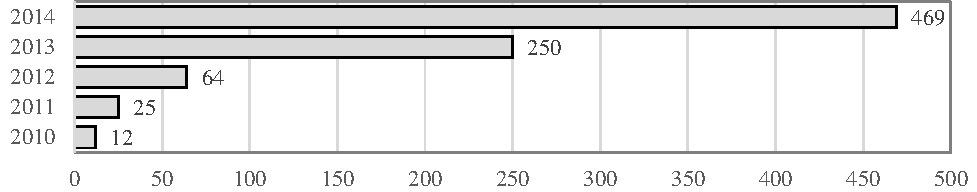
\includegraphics[width=.90\textwidth]{crawl-Zeit1-sicherhheit_cropped.pdf}
\caption{Zeitliche Aufteilung der Zeitungsartikel}
\label{fig:url-found}
\end{figure}

Die Auswahl der Zeitungsartikel erfolgte durch eine zufällige chronologische Stichprobenziehung durch eine Programmierung in Python 2.7.6. Ausgehend von der Indexhomepage der Zeitung ZEIT ONLINE wurde am 1. März 2014 ein rekursives Hyperlinksammelverfahren verwendet. Folgendes ist dabei anzumerken: Durch das rekursive Vorgehen fand der Algorithmus eine höhere Anzahl an aktuellen Artikeln. Je älter die Artikel waren, desto unwahrscheinlicher war das Auffinden der Anzahl gemäß gering referenzierten älteren Artikeln. Die Verteilung des Erscheinungsjahres der Artikel kann Abbildung~\ref{fig:url-found} entnommen werden. Dieses rekursive Verfahren führte dazu, dass n = 820 Hyperlinks gefunden wurden, die auf einen Zeitungsartikel verwiesen.\footnote{Durch das automatisierte Verfahren wurden zu Beginn N = 6.800 Hyperlinks gefunden, die nach einer manuellen Begutachtung auf n überprüfte Hyperlinks bereinigt wurden.} In dem folgenden Schritt wurden die manuell überprüften Hyperlinks wiederholt eingelesen, um den Titel, das Publikationsdatum, die Anzahl der Kommentare und die Hauptkategorie des Artikels zu extrahieren. 

In dem darauf folgenden Schritt wurden die einzelnen Kommentare von vier ausgewählten Zeitungsartikeln ausgelesen.  Dabei wurden Artikel aus verschiedenen Themenbereichen gewählt, die eine vergleichbar hohe Anzahl an Kommentaren aufwiesen. Dabei stellte der folgende Reguläre Ausdruck die Basis des Programms. Auf Basis der einzelnen Kommentare wurde eine Datenbank erstellt.

\begin{footnotesize}
\begin{minted}{python}
pattern = '([^><]+)(?<!Leserempfehlungen)(?<!anzeigen)(?<!. )<[^<]+>'
com = [re.findall(pattern,comment) for comment in rawcomments]
\end{minted}
\end{footnotesize}



\subsection{Deskriptive Statistik}
Die Analyse der Daten wurde in zwei Abschnitte aufgeteilt. In der Metaanalyse steht die Gesamtheit der kommentierten 820 Artikel im Vordergrund. Es wurden vier Artikel ausgewählt, die statistische Ausreißer darstellten. Mit Hilfe einer qualitativen als auch quantitativen Analysen werden mögliche Methoden zur Untersuchung von einzelnen Artikeln im folgenden Abschnitt bewertet.

%\subsubsection{Metaanalyse}

\begin{figure}[h!]
%\centering
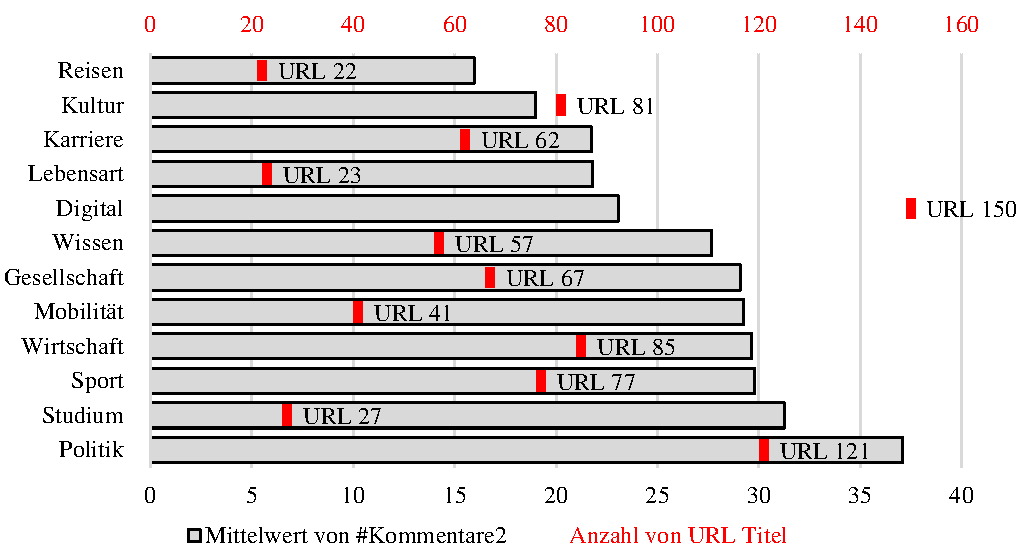
\includegraphics[width=.90\textwidth]{km_kt.pdf}
\caption{Kategorien der Zeitungsartikel}
\label{fig:kommentar-kategorie}
\end{figure}

Um den Datensatz zu kontrollieren wurden zwei Validierungsverfahren angewendet. Da von ZEIT ONLINE verschiedene Hauptkategorien verwendet werden, wurde überprüft, ob die Anzahl der Hyperlinks je Kategorie grundsätzliche statistische Implikationen zulassen kann. Zweitens wurde qualitativ
überprüft, ob die durchschnittliche Anzahl der Kommentare je Kategorie realitätsnah und somit ohne technische Fehler ist. In Abbildung~\ref{fig:kommentar-kategorie} ist diese Überprüfung grafisch veranschaulicht.

Ein weiteres qualitatives Validierungsverfahren der Stichprobe bestand in der Analyse des Veröffentlichungsdatums. Dabei wurde angenommen, dass ZEIT ONLINE durch die normalen Beschäftigungsverhältnisse mehr Artikel während der Woche veröffentlicht, als es an Samstagen und Sonntagen der Fall ist. Diese Analyse wurde gleichzeitig mit der durchschnittlichen Anzahl von Kommentaren je Artikel an einem bestimmten Wochentag kombiniert. Diese Analyse ist in Abbildung~\ref{fig:kommentar-wochentag} dargestellt.

\begin{figure}[h!]
%\centering
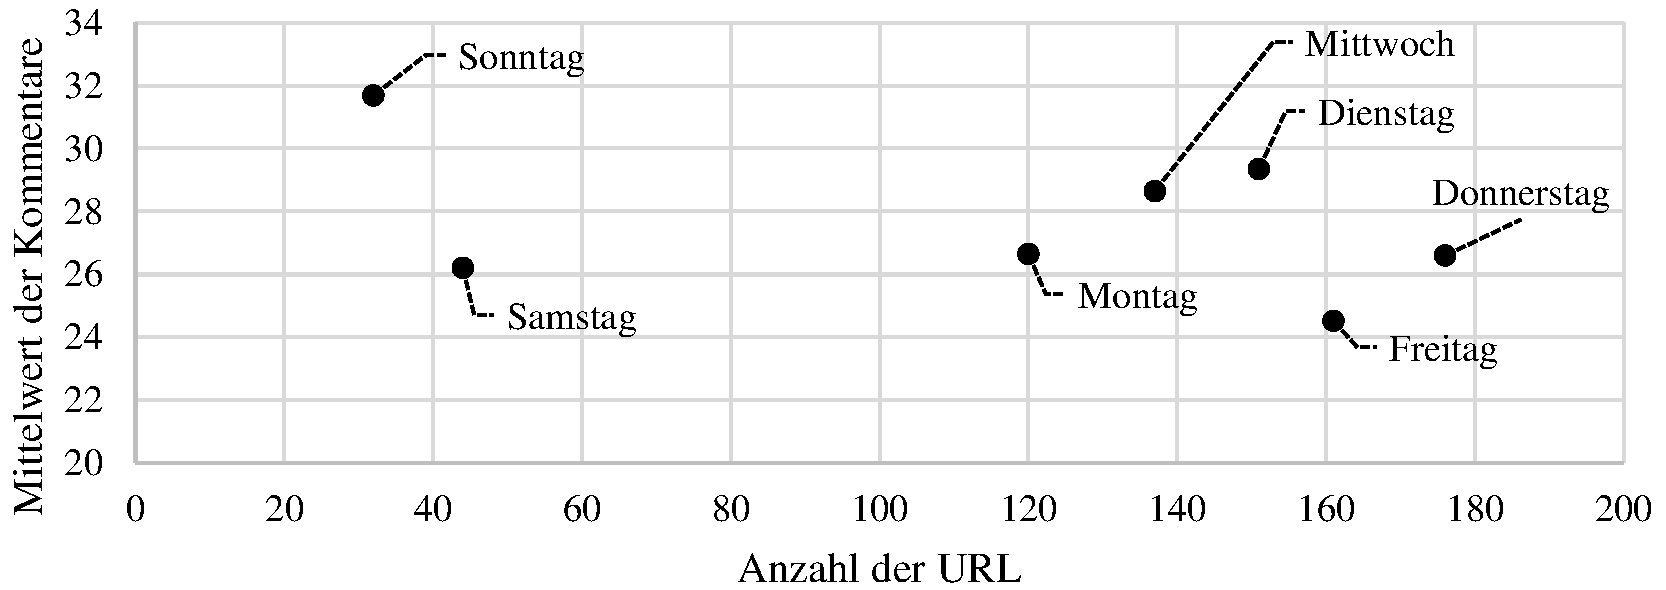
\includegraphics[width=.90\textwidth]{Kom_Wt.pdf}
\caption{Publikationsdatum nach Wochentagen}
\label{fig:kommentar-wochentag}
\end{figure}

\newpage
%\subsubsection{Kommentaranalyse}

\begin{footnotesize}
\begin{minted}{python}
words = "Textstring"
words = [word for word in words if word.isalpha()]
diff_words = set(words)
diversity = len(diff_words) / float(len(words))
print diversity
\end{minted}
\end{footnotesize}

%{strukturelle Analyse: lexikalische Diversität}\\

% Nun kann man auch ganz einfach die Diversität für Mobby Dick oder die anderen Texte berechnen. Die Diversität ist ein Maß für die Sprachvielfalt. Sie ist definiert als Quotient der “verschiedenen Wörter” dividiert durch die “Gesamtanzahl von Wörtern” eines Textes.

Im ersten Schritt der Kommentaranalyse wurde der oben genannte Algorithmus erstellt. Dabei wurde die Anzahl der nicht identischen Wörter mit der Gesamtanzahl der Wörter verglichen. So ergab sich zum Beispiel bei dem Ukraine Artikel ein Wert von 0,00027 \cite{Greven2014Zeit}. Um diese Zahl bewerten zu können, wurden mit dem oben genannten Algorithmus Vergleichswerte von bekannter Standartliteratur errechnet. Die Werte können in Tabelle~\ref{tab:sprachliche_div} nachgelesen werden. Auf Basis dieser Vergleichswerte konnte festgestellt werden, dass eine hohe sprachliche Diversität in den Kommentaren vorherrscht. Diese hohe sprachliche Diversität lässt sich durch stark fehlerhafte Orthographie begründen.

%# Quelle: http://update.hanser-fachbuch.de/2013/09/artikelreihe-python-3-nltk-natural-language-toolkit/

%%%%%% Beginn von der Tabelle
\begin{singlespace}
\captionof{table}{Vergleich lexikographischer Diversität}
\label{tab:sprachliche_div}
\noindent\begin{tabularx}{.90\textwidth}{l|l} %140mm astatt \textwidth
    % Das X steht oben für die Spalte, die automatisch and die Seitenbreite angepasst werden soll!!
    \hline
    \textbf{Quelle} & \textbf{Index}  \\ \hline 
Moby Dick, Herman Melville 1851                                                               & 0,09             \\
Sense and Sensibility, Jane Austen 1811                                                       & 0,06             \\
The Book of Genesis                                                                             & 0,07             \\
Inaugural Address Corpus                                                                        & 0,07             \\
Chat Corpus                                                                                     & 0,15             \\
Monty Python and the Holy Grail                                                                 & 0,18             \\
Wall Street Journal                                                                             & 0,13             \\
Personals Corpus                                                                                & 0,29             \\
The Man Who Was Thursday, G. K. Chesterton 1908                                             & 0,12             \\
\end{tabularx}

\end{singlespace}
%%%%% Ende der Tabelle  




%{Konnotierte Wort Analyse}\\


Durch die von Rechtschreibfehlern und weiteren Besonderheiten der Textverfassung (z. B. die häufige Verwendung von "....") geprägten Schreibweisen, wurde von einer emotionalen Textanalyse abgesehen. Diese Analyse ermöglicht auf Basis von einem bereits existierenden Datensatz die Zählung emotional konnotierter Wörter \cite{BAWLR}. Außerdem kann der Datensatz genutzt werden, um  Wörter auf ihre positive oder negative Konnotation zu bewerten. Verschiedene bereits erprobte Verfahren können angewendet werden, um den emotionalen Verlauf der Diskussion zu bewerten \cite{vo2006cross,vo2009berlin}.

Um der individuellen Orthographie Rechnung zu tragen, wurden vier weiter Methoden genutzt, um die  vier selektieren Kommentare zu bewerten. Ausgehend von der Frage nach der sprachlichen Vielfalt in den Kommentaren wurde der Diskussionsverlauf eines Artikels analysiert \cite{eemueller}. Dabei wurde die Anzahl der Nennungen eines Wortes untersucht und grafisch abgetragen (Abbildung~\ref{fig:python-worddensity}). Es fiel auf, dass Fragezeichen (\textit{?}) häufiger verwendet werden als Ausrufezeichen (\textit{!}). Diese Zählung wurde anschließend für alle Kommentare wiederholt. Es war festzustellen, dass die Auftrittswahrscheinlichkeit von Fragezeichen (\textit{?}) in einem Kommentar in jedem der Fälle die Auftrittswahrscheinlichkeit von Ausrufezeichen (\textit{!}) überstieg. Eine qualitative Textanalyse ergab, dass sich vermehrt rhetorische Fragen in den Kommentaren finden. Die genauen Auftrittswahrscheinlichkeiten können Tabelle~\ref{tab:?!-auftritt} entnommen werden.

\newpage

\begin{landscape}
\begin{figure}[h!]
%\centering
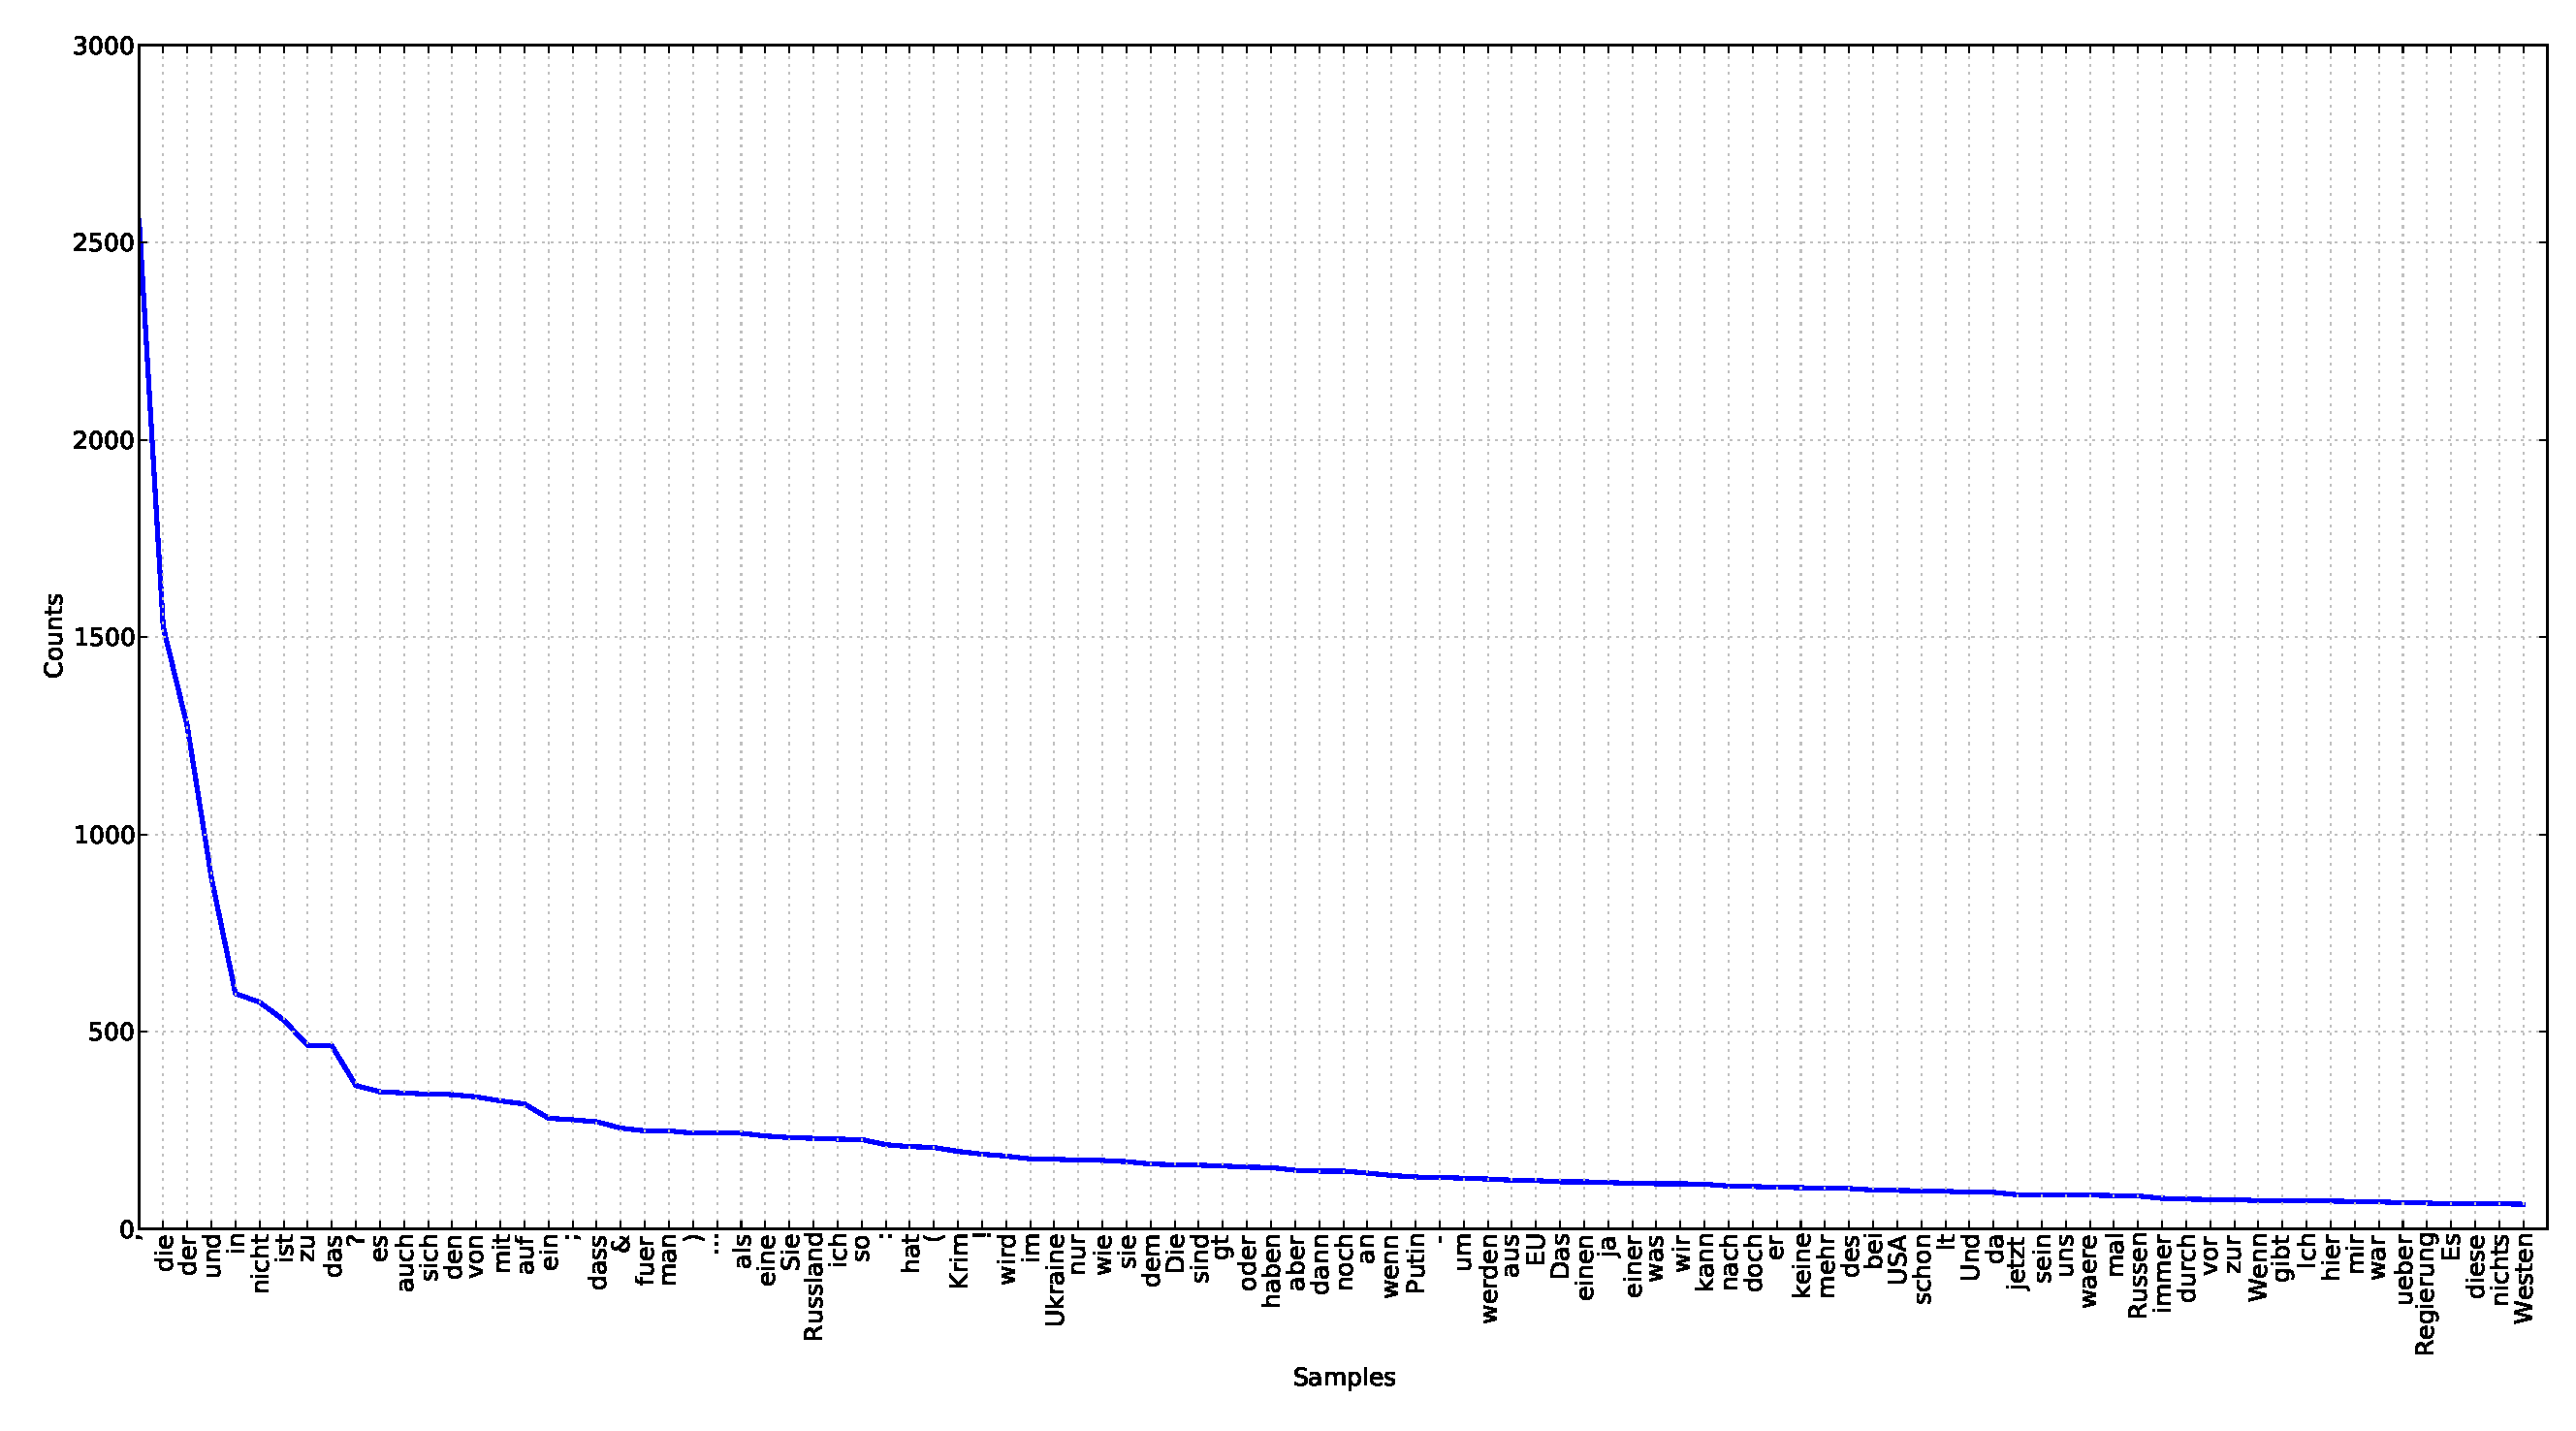
\includegraphics[height=.85\textheight]{100_most_kommentar-text.pdf}
\caption{Häufigkeit der Wörter in Kommentaren}\cite{Greven2014Zeit}
\label{fig:python-worddensity}
\end{figure}
\end{landscape}
\newpage

 
%%%%%% Beginn von der Tabelle
\begin{singlespace}
\captionof{table}{Auftrittswahrscheinlichkeit eines ? oder ! je Kommentar}
\label{tab:?!-auftritt}
\noindent\begin{tabularx}{.90\textwidth}{l|l|l|l} %140mm astatt \textwidth
    % Das X steht oben für die Spalte, die automatisch and die Seitenbreite angepasst werden soll!!
   
    
    
    \hline
    \textbf{Artikel} & \textbf{Anzahl der Kommentare}  & \textbf{?}    & \textbf{!}           \\ \hline 


Burka               & 209                   & 71\%  & 31\%        \\
Downsyndrom         & 189                   & 67\% & 21\%        \\
Teilzeit für Eltern & 136                   & 48\% & 40\%        \\
Ukraine             & 581                   & 62\% & 32\%           \\       
\end{tabularx}
\end{singlespace}

Aus der grafischen Analyse in Abbildung~\ref{fig:python-worddensity} kann entnommen werden, dass die häufigsten Nomen (Russland, Krim, EU, Westen, Regierung) den Inhalt des ursprünglichen Artikels widerspiegeln \cite{Greven2014Zeit}. Diese Häufigkeits\-verteilung von charakteristischen Nomen in den Diskussionen, konnte darüber hinaus auch in den restlichen Artikeln gefunden werden. So kam das Wort \textit{Frauen} 178 Mal in den Burka Kommentaren \cite{Sadigh2014Zeit}, \textit{Teilzeit} 28 Mal in den Teilzeit Kommentaren \cite{Zeit-2-2014Zeit}, \textit{Russland} 230 Mal in den Ukraine Kommentar \cite{Greven2014Zeit} und \textit{Kind} 140 Mal in den Downsyndrom Kommentaren \cite{Wezel2014Zeit} vor.

Neben den ersten beiden Methoden zur Analyse des Inhalts wurden zwei weitere Methoden zur Untersuchung der Länge und der Anzahl der Beiträge verwendet. Im dem ersten Schritt wurden die Kommentare je Artikel den jeweiligen Nutzernamen zugeordnet \cite{Greven2014Zeit}. Mit Hilfe einer Lorenzkurve wurde die (Ungleich-)Verteilung der Länge und Anzahl der Beiträge auf die Nutzer untersucht (Abbildung~\ref{fig:lorenz-kommentar}). Dabei fiel auf, dass eine kleine Gruppe von Nutzern einen hohen Beitrag an der gesamten Diskussion einnahmen (Gini-Koeffizient = 0,69). 
\section{Model}
Zweitens wurde die Textlänge der Kommentare untersucht, ohne diese den Internetnutzern zuzuordnen. Die Textlänge wurde als Häufigkeitsverteilung in Abbildung~\ref{fig:kommentar-density} abgetragen. Dabei konnte festgestellt werden, dass die Verteilung signifikant rechtsschief ist. Es ist jedoch anzumerken, dass in jeder der vier Diskussionen eine Gruppe von Beiträgen mit langer Textlänge zu finden ist. Die Dichtefunktion fällt in dem Intervall 1000 bis 1900 Zeichen nicht monoton ab, sondern steigt kurzzeitig an. Obwohl diese Anomalie der Verteilung nicht signifikant ist, wurden zwei Diskussionen ausgewählt. Auf diese Weise konnte durch die Verbindung von qualitativem und quantitativem Vorgehen die Verlässlichkeit der Analyse gestärkt werden. Bei den Artikeln über die Ukraine und über ein Teilzeitmodell für Eltern fiel eine ausgeprägte Gruppe von langen Textbeiträgen auf. Bei dem Artikel über das Teilzeit\-modell für Eltern stellt diese Gruppe der längeren Kommentare ausführlich die persönliche Lebenssituation dar \cite{Zeit-2-2014Zeit}. Dieses Thema macht es möglich, dass die Kommentierenden neben ihrer Meinungen einen persönlichen Einblick geben können. Die meisten Nutzer, die einen Kommentar mit einer langen Textlänge schrieben, verfassten lediglich einen Kommentar und kehrten nicht zu der Diskussion zurück. In dem zweiten Artikel konnte festgestellt werden, dass die Gruppe der längeren Kommentare eine sich gegenseitig referenzierende Diskussion darstellt \cite{Greven2014Zeit}. So haben die Kommentierenden \textit{Jemand der kommentieren will} und \textit{Zivilisationswächter} einen Anteil von 7,43 \% der Textlänge an der gesamten Diskussion.

\begin{figure}[h!]
%\centering
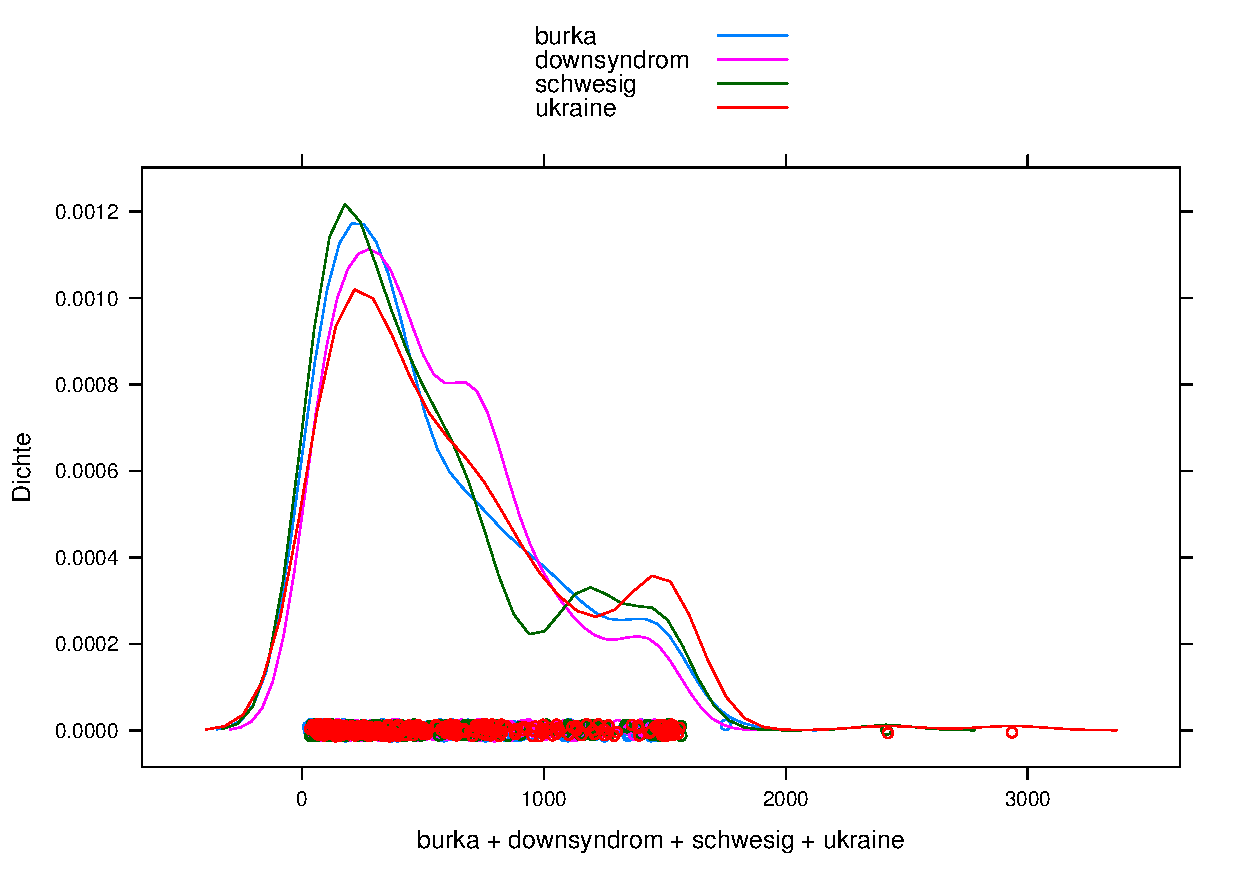
\includegraphics[width=.90\textwidth]{density_textlaenge.pdf}
\caption{Verteilung der Länge der Kommentare}
\label{fig:kommentar-density}
\end{figure}


%Verteilung auf Kommentierende, Gini-Koeffizient	0,692216015


\newpage
\begin{landscape}
\begin{figure}[h!]
%\centering
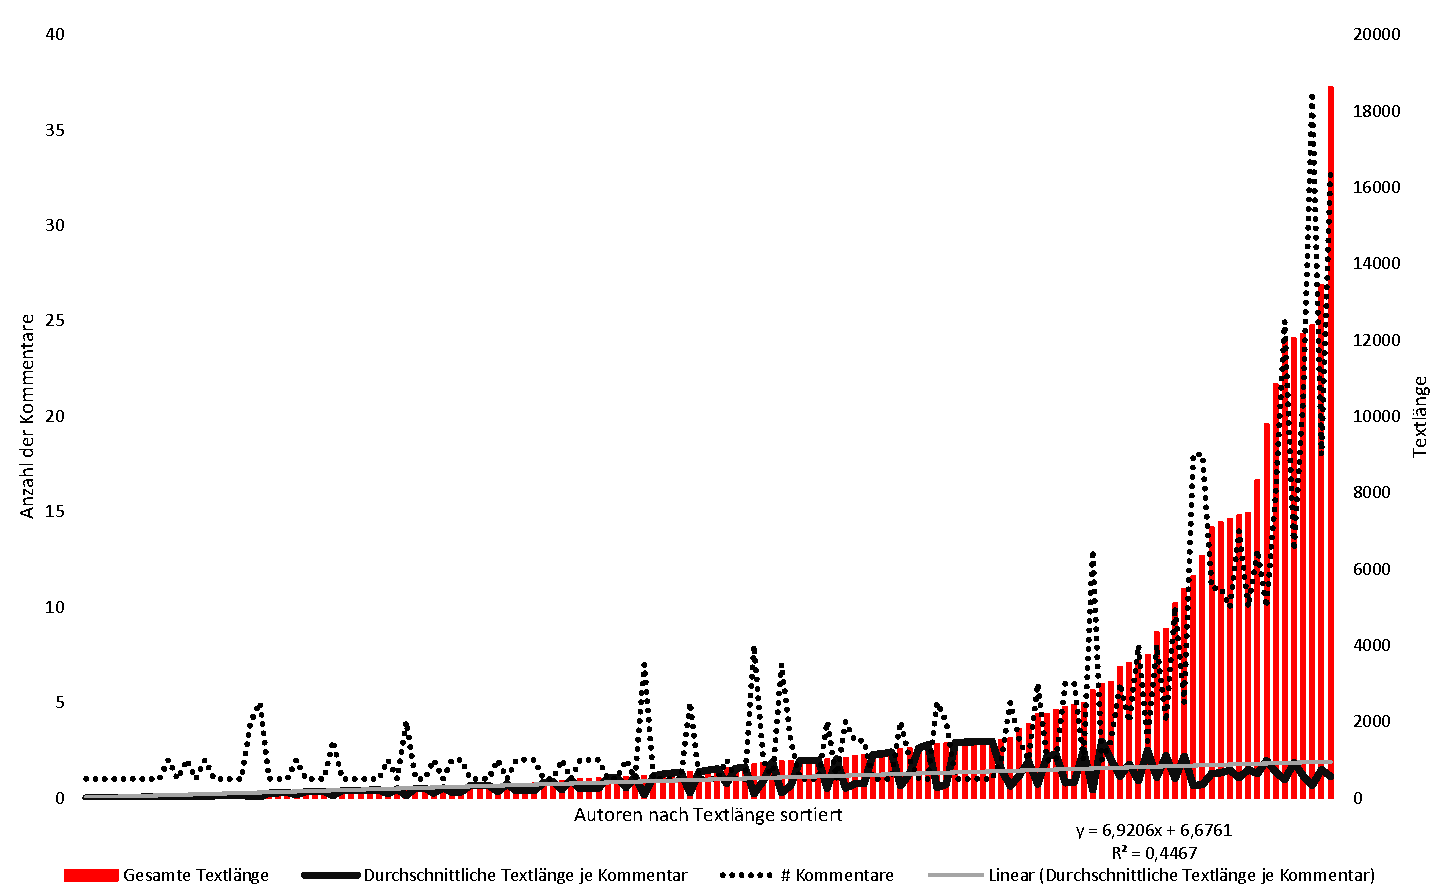
\includegraphics[height=.85\textheight]{erste_Artikelauswertung_cropped.pdf}%
\caption{Zeitliche Aufteilung der Zeitungsartikel}
\label{fig:lorenz-kommentar}
\end{figure}
\end{landscape}
\newpage


\newpage
\section{Ergebnisse}
\subsection{Arbitrage}
\subsection{Dominante Trading Strategien}
\subsection{Preissetzung durch Amazon}


%\subsection{Inhaltliche Erkenntnisse der Methoden}
Der Wochenverlauf hat keinen signifikanten Einfluss auf die Interaktion der Kommentierenden. Denn die Anzahl der durchschnittlichen Kommentare je Artikel, die an einem Wochenende publiziert werden, unterscheidet sich nicht signifikant von anderen Artikeln (Abbildung~\ref{fig:kommentar-wochentag}). Auch die Anzahl der ver\-öffentlich\-ten Artikel pro Tag haben keinen signifikanten Einfluss auf die durchschnittliche Anzahl der Kommentare je Artikel (Abbildung~\ref{fig:kommentar-wochentag}). Die Anzahl verfüg\-bar\-er Artikel hat keinen Einfluss auf die durchschnittliche Anzahl der Kommentare (Abbildung~\ref{fig:kommentar-kategorie}).

Sowohl die konstante Interaktionshäufigkeit (Abbildung~\ref{fig:kommentar-wochentag}) als auch das themenübergreifende Interesse (Abbildung~\ref{fig:kommentar-kategorie}) zeigt ein freiwilliges Interesse seine Ansichten zu teilen. Die Leistung der Kommentierenden kann durch die zum Teil sehr ausführliche Darstellung der eigenen Meinung als ausführlich bewertet werden \cite{williams1998demography}. Hypothese II kann dabei nicht signifikant belegt werden (p-Wert $\geq$ 0,05).

Die signifikant rechtsschiefe Verteilung der Beiträge sowie ein Gini-Koeffi\-zient von 0,69 stützen Hypothese I nicht. Die ungleichmäßige Verteilung kann sogar in zwei Gruppen aufgeteilt werden (Abbildung~\ref{fig:kommentar-density}). Die Kommentare mit einer langen Textlänge hängen nicht unmittelbar mit dem Gesamtbeitrag des jeweiligen Kommentierenden zusammen. So haben viele Frauen in dem Artikel über Elternteilzeit in einem einzigen Kommentar ihre persönliche Situation geschildert \cite{Zeit-2-2014Zeit}. Demgegenüber haben in dem Artikel über die Ukraine wenige Kommentierende eine stark autarke Diskussion geschaffen, indem sie sich gegenseitig referenzierten \cite{Greven2014Zeit}.

\section{Vergleich mit anderen Erklärungsansätzen}

Hypothese III konnte sowohl quantitativ (Abbildung~\ref{fig:python-worddensity}) als auch qualitativ überprüft werden. Ausgehend von Hypothese III konnte darüber hinaus eine hohe Interaktion zwischen den Nutzern festgestellt werden (Tabelle~\ref{tab:?!-auftritt}). Die Anzahl der häufigsten Nomen in einer Diskussion eines Artikels scheinen auffällig mit dem Thema des Artikels in Verbindung zu stehen (Abbildung~\ref{fig:python-worddensity}). Die Anzahl der Fragezeichen überwiegt die Anzahl der Ausrufezeichen (Tabelle~\ref{tab:?!-auftritt}). Eine besondere Häufigkeit von rhetorischen Fragen konnte gefunden werden. Dieses Resultat konnte nicht statistisch überprüft werden.

\subsection{Marketing durch Händler}
\subsection{Informationskosten}
\subsection{Erlebnisfaktoren für private Verkäufer}
\subsection{Mental Accounting}
Das explorative Vorgehen hat es ermöglicht verschiedene Methoden zur Analyse der Kommentierenden der ZEIT ONLINE zu untersuchen. Grundsätzlich führen Verfahren, die eine semantische Analyse des Texts vornehmen durch die hohe Anzahl der orthographischen Fehler zu einem nicht reliablen Ergebnis. So ist zum Beispiel die Messung von sprachlicher Diversität abhängig von der Anzahl der orthographischen Fehler. Somit konnte die sprachliche Diversität nicht überprüft werden. Das Verfahren zur Bestimmung der emotionalen Konnotation ist validiert, konnte jedoch aus genannten Gründen nicht eingesetzt werden \cite{vo2006cross,vo2009berlin}.

Alle verwendeten Analysen in dem ersten Abschnitt der Datenanalyse konnten ohne Beschränkung angewendet werden. Drei gefundene Verfahren ermöglichen es einen qualitativ validierbaren Einblick in die einzelnen Kommentare zu erhalten. Mit diesen Verfahren kann sowohl die Verwendung von Nomen, Ausrufezeichen und Fragezeichen dargestellt werden. Die Häufigkeits\-verteilung und die Lorenzkurve beschreiben die Beteiligung der Kommentierenden unabhängig von dem Inhalt der Beiträge. Diese Eigenschaft macht die Ergebnisse der beiden Verfahren hinreichend robust.

\newpage
\section{Diskussion}
\subsection{Implikationen für die Theorie}
Die Erweiterung der Definition von Diversität hat diese explorative Studie und den Datenzugang ermöglicht. Die Studie konnte isoliert die intelektulle Diversität in einem bereits beschriebenen Kontext analysieren. Daten zu Äußerungen von Personen können auf diese Weise ohne Befragung erlangt werden \cite{joshi2009role,jackson2003recent}. Die Personen werden nach Ihrer Aktivität auf Grund ihrer verbalen Artefakte in Form von Texten analysiert. Auf diese Weise kann einer Messverzerrung durch Beobachtung vorgebeugt werden \cite{ruso2007qualitative}. Unangemessene Äußerungen müssen bei diesem Datenmaterial nicht nachträglich bereinigt werden, da dies bereits durch den Betreiber der Plattform geschieht \cite{kiesler1984social,siegel1986group}. Die anonyme Diskussion reduziert den Einfluss der \textit{Sozialen Rolle} der Partizipierenden \cite{dey2001understanding}.

Es konnte nicht belegt werden, dass Beiträge einer \ac{CMC} Diskussion gleich\-mä\-ßig auf die Gruppenmitglieder verteilt sind \cite{siegel1986group,mcguire1987group}. In den Kommentaren konnte jedoch eine hohe inhaltliche Nähe zu den Artikeln festgestellt werden. Die Aktivität der Nutzer ist dabei über die Woche konstant.

Diversität kann durch fehlende Metadaten der Kommentierenden auf Basis der momentanen Methoden trotz Hilfsmitteln der Computerlinguistik nicht operationalisiert und nicht nachgewiesen werden \cite{lawrence1997perspective,lapid1998diversity,harrison1998beyond,harrison2007s}. Der Nachweis lässt sich auf Basis der Daten nur qualitativ begründen. 

Die Analyse hat gezeigt, dass die Kommentierenden einen Teil ihrer persön\-lichen Attribute zugänglich machen \cite{van2004work,vashanti2012}. Gleichzeitig konnte keine freiwillige organisationale Aktivität von ZEIT ONLINE beobachtet werden, die darauf gerichtet war einen höheren Grad der Inklusion von Individuen auf formaler oder informeller Ebene zu erreichen \cite{gilbert1999dm,ewoh2013}. 

 

\subsection{Implikationen für die Praxis}
Die Informationsfunktion der Zeitung ZEIT ONLINE ist in dem CMC Kontext erweitert aufzufassen \cite{neuberger1999online}. Es konnte festgestellt werden, dass die Online-Diskussionsplattform ausgiebig genutzt wird. Der Verlauf und die Ergebnisse der Diskussion werden jedoch bisher nicht von ZEIT ONLINE aufgegriffen. Die Öffnung des Unternehmens gegenüber der intellektuellen Diversität der Nutzer, könnte zugleich ein Vorteil für das Unternehmen in dem Wettbewerbsmarkt der Medien sein \cite{gassmann2006open,stachbert,enkel2014applying}. Die aufgezeigte bestehende Diversität der Nutzer kann es ermöglichen eine firmeninterne Diversitätssteigerung zu erreichen. Ein solches Open Diversity Management kann wie folgt aussehen:

ZEIT ONLINE kann sich gegenüber den aktiv Kommentierenden öffnen und deren Ideen, Erfahrungen und Meinungen in die eigene publizierte Meinung integrieren. Dies kann sowohl methodische als auch inhaltliche Änder\-ungen der Kommentarfunktion bedeuten. Einerseits besteht die Möglichkeit eine automatische Rechtschreibprüfung zu integrieren, um eine spätere Textanalyse durch das Unternehmen zu vereinfachen. Außerdem können direkte Verbindungen zu dem Text des Artikels zugelassen werden. Momentan kann ZEIT ONLINE nicht feststellen, welcher Kommentar sich auf welche Passage des Zeitungsartikels bezieht. Diese Verknüpfung kann zukünftig dazu genutzt werden sensible Themenbereiche zu identifizieren, um vor der Erstellung eines Artikels nutzerzentrierte Schwerpunkte festzulegen. Gleichzeitig haben Leser (durch die Verbindung zu Textstellen des Artikels) direkten Einblick auf relevante Kommentare der soeben gelesenen Passage. Ein Aufblenden der verknüpften Kommentare bei der Markierung mit der Computer-Maus könnte ein Beispiel sein.\footnote{Diese Funktion wird von www.soundcloud.de für Musik angeboten.}

Darüber hinaus besteht die Möglichkeit das hohe Interaktionsvolumen von wenigen Nutzern zu honorieren. So kann eine verlinkte Seite für den Artikel von ZEIT ONLINE erstellt werden, auf dem ein ausgewählter Kreis von Nutzern gemeinschaftlich einen Kommentar oder eine Rezension schreiben. Außerdem hat es ZEIT ONLINE bisher noch nicht ermöglicht, Betreiber von verschiedenen Blogs zu integrieren. So könnte die Meinungsvielfalt und Offenheit von ZEIT ONLINE ansteigen, indem auf Blogeinträge verwiesen wird, die im Zusammenhang mit dem jeweiligen Zeitungsartikeln stehen. Die Auseinandersetzung der Redakteure mit gegenwärtigen Entwicklungen in der virtuellen Meinungsbildung kann auf die beschriebenen Weisen die Diversität des gesamten Unternehmens kostengünstig steigern und gleichzeitig die Kundenbindung erhöhen.

\subsection{Limitationen und weitere Forschung}
Der Theorieteil hat gezeigt, dass Personen bei der Verwendung von anonymen Nutzerprofilen ihre Meinung besonders ungehemmt darstellen. Verhaltensweisen von Personen, die das Benutzerprofil bei ZEIT ONLINE mit dem eigenen Namen personalisiert haben, konnten auf Basis der Daten nicht mit Personen, die vollständig anonym kommmentierten, verglichen werden. Die Aussagen über das Verhalten der Kommentierenden kann bisher nicht auf andere Zeitungen oder Online-Plattformen erweitert werden. Falls ZEIT ONLINE\- besonders viele aktive Nutzer im Vergleich zu ähnlichen Plattformen hat, sollte analysiert werden, welche Möglichkeiten ZEIT ONLINE bietet, die das hohe Nutzerverhalten erklären. Darüber hinaus war das Vorgehen der Studie explorativ. Trotz größter Sorgfalt besteht die Möglichkeit weitere Methoden zu finden, die bisher nicht belegbare Aussagen überprüfen können.

Für die weitere Analyse des Open Diversity Managements ergeben sich verschiedene Fragen. Grundsätzlich gilt es zu klären, ob eine Übertragung des Open Innovation Gedankens grundsätzlich zulässig ist. In dieser Arbeit können Gründe für eine Integration der Meinungsvielfalt in das Unternehmen ZEIT ONLINE gefunden werden. Es kann jedoch nicht geklärt werden, ob dies in anderen Branchen außer in der Medienbranche diversitäts- bzw. wettbewerbsfördernd ist. Darüber hinaus wird es hilfreich sein zu fragen, welchen Einfluss ein diverses Umfeld auf das Unternehmen hat. Unabhängig von dem Gedanken des Open Diversity Managements fordert die anonyme Umgebung des Internets eine weitere Operationalisierung von Diversität. Diese Operationalisierung sollte bestenfalls ein Diversitätspotential einer anonymen Masse für Unternehmen bewerten können.


%%%%%%%%%%%%%%%%%%%%%%%%%%%%%%%%%%%%%%%%%%%%%%%%%%%%%%%%%%%%%%%%%%%%%%%%%%%%%%%%%%%%%%%%%%%%%%%%%%
%%%%%%%%%%%%%%%%%%%%%%%%%%%%%%%%%%%%%%%%%%%%%%%%%%%%%%%%%%%%%%%%%%%%%%%%%%%%%%%%%%%%%%%%%%%%%%%%%%
%                    Hier endet das echte Dokument!!!
%%%%%%%%%%%%%%%%%%%%%%%%%%%%%%%%%%%%%%%%%%%%%%%%%%%%%%%%%%%%%%%%%%%%%%%%%%%%%%%%%%%%%%%%%%%%%%%%%%
%%%%%%%%%%%%%%%%%%%%%%%%%%%%%%%%%%%%%%%%%%%%%%%%%%%%%%%%%%%%%%%%%%%%%%%%%%%%%%%%%%%%%%%%%%%%%%%%%%

\newpage
\section{Bibliographie}

\bibliographystyle{apsr}

\bibliography{references}

\normalsize
\newpage
\section{Appendix}
\subsection{Webcrawler}
\begin{minted}{python}
# -*- coding: cp1252 -*-
##import urllib
##import lxml.html
##
##
##sock = urllib.urlopen("http://www.zeit.de/politik/ausland
/2014-03/ukraine-krim-russland-militaer-intervention?
commentstart=9#comments") 
##htmlSource = sock.read()                            
##sock.close()                                       
###print htmlSource
##
##
##with open("temp\Article.txt","w") as text_file:
##    text_file.write(htmlSource)
##
##with open("temp\Article.txt","r+") as Article:
##    data = Article.read()
##    
##
##x = data.split('"')
##
##with open("temp\stings.txt","w") as Strings:
##    Strings.write(x)
##
##
##    
##    
##    
    
import codecs
import urllib
htm = urllib.urlopen("http://www.zeit.de/politik
#/deutschland/2014-02/freihandelsabkommen-goering-
#eckhardt-transparenz")

#z = htm.read().decode('utf-8')
z = htm.read()


#number = text[text.find("<a href='#comments' title='' 
itemprop='interactionCount' content='UserComments:")+1:
text.find("Kommentar")]

#z = '<a href="#comments" title=""
itemprop="interactionCount" content="UserComments:187">
187 Kommentare</a>'
s = z[z.find('<a href="#comments" title="" 
itemprop="interactionCount" content="UserComments:')+79:
z.find(' Kommentare</a>')+1]
# u ist der Teil des Vektors der #von Kommentaren
u,w = s.split('"')
print u
#Kategorien und Artikelueberschrift
#breadsplit = breadcrump[breadcrump.find('<span itemprop="title">')
:breadcrump('</span></a></li>')]

header = z[z.find('<h1>'):z.find('</h1>')]
print header
date = z[z.find('<span class="articlemeta-left"><span 
class="articlemeta-datetime">')+66:z.find('</span></span>
<span class="articlemeta-right">')]
cdate, r = date.split('\xc2\xa0\n\t\t\t\t\t\t\t\t\t')
print cdate

#Kurzbeschreibung
#k1 = z[z.find('<meta property="og:description" content=')+40:
z.find('</span></span><span class="articlemeta-right">
<span class="articlemeta-toolsbutton"')-3]
\end{minted}
\subsection{Auktionen extrahieren}

\begin{minted}{python}

# -*- coding: utf-8 -*-

import doctest

#################################################################
#################################################################
# Leserlichkeit von Texten nach Flesch
#################################################################
#################################################################

from re import *


class Flesch(object):
    def __init__(self,text):
        self.text = text


    def anzahlWorte(self):
        return len(self.text.split())

    def anzahlSaetze(self):
        re = compile('[!?.;:]+\s')
        return len(re.split(self.text))

    def anzahlSilben(self):
        re = compile('[aeiou]+',I)
        return len(re.split(self.text))

    def readability(self):
        asl = float(self.anzahlWorte())/self.anzahlSaetze()
        asw = float(self.anzahlSilben())/self.anzahlWorte()
        return int(206.835-1.015*asl-84.6*asw)

    def __str__(self):
        return 'Lesbarkeitsindex nach Felsch: '+\
               str(self.readability())

#################################################################
#################################################################
# URL Existenz
#################################################################
#################################################################

def urlexist(url):
    """
    Given typine x(), return kk.
    >>> x()
    'kk'
    """
    import urllib2, urllib
    try:
        f = urllib2.urlopen(urllib2.Request(url))
        urlok = True
    except:
        urlok = False
    return urlok

#################################################################
#################################################################
# HTML von einer URL UTF-8 kodieren und Tabs und Umbruch delete
#################################################################
#################################################################

def html_utf8(url):
    import urllib, codecs
    if urlexist(url):
        #print "URL ok"
        html = urllib.urlopen(url).read()
        html = unicode(html,'utf-8')
        html = html.replace("\n","").replace("\t","")
    else:
        html = url,"URL does not exist!"

    return  html

#################################################################
#################################################################
# Kommentare
#################################################################
#################################################################


def zeitcomments(html):
    import re
    try:
        # cut begin away
        htmlcut1 = html.split("<ol>")
        htmlcut1 = htmlcut1[1]
        # cut end away
        htmlcut2 = htmlcut1.split('</div></li></ol>')
        rawcomments = htmlcut2[0]
        # Zeilenumbueche die von Nutzern in Text 
        
        rawcomments = rawcomments.replace('<br>','').
        replace('<p>','').replace('</p>','').replace('<em>','').
        replace('<br />','')
    except:
        print "Fehler bei HTML Cut"
        result = False
    pattern ='<a title="Vorw[^"]+rts" class="fwd" href="([^"]+)">'
    nexturl = re.findall(pattern,html)
    try:
        nexturl = nexturl[0] # falls mehrere gleich 
        #Links gefunden werden
    except:
        nexturl = False

    rawcomments = rawcomments.split('<ul class="user">')
        
    
    rawcomments = rawcomments[1:]
 
    pattern = 'cid-(\d{4,})">.{0,}</a>'
    ID = [re.findall(pattern,comment) for comment in rawcomments]
    pattern = '([^><]+)(?<!Leserempfehlungen)
    (?<!anzeigen)(?<!. )<[^<]+>'
    com = [re.findall(pattern,comment) for comment in rawcomments]

    people = len(com)
    
    for people in range(people):

                 
        
        # Wenn 8 Elemente, dann 5tes und 6tes mit 4 tem verbinden
        # Wenn 5 Elemente komplett leoschen
        # Wenn 7 Elemente, dann 5tes mit 4 tem verbinden
        # wenn neun Elemente, dann 4+5+6 verbinden
        
        try:
            if len(com[people][3])>300:
                # Flesch Readability berechnen
                x = Flesch(com[people][3]) # Achtung NEU
                readability = x.readability()    #Achtung NEU               
            else:
                readability = "Article too short"
        except:
            readability = "no text found"

        # "Redaktion" suchen, dummy variable

        """
        noch offen
        """
                            

        # Fuellwoerter zaehlen
        """
        noch offen
        """

        # Ausgabe durch print in Shell, Bewertung von
        ## Separation, Variety and Disparity durch Nutzer

        """
        noch offen
        """

        com[people] += ID[people], readability
 
            
   
    else:
        print  "Seite mit ",people," Kommentaren ausgelesen"

    # Return Result
    return com, nexturl


#################################################################
#################################################################
# Write CSV
#################################################################
#################################################################

def writecsv(listobject):
    import csv
    with open('E:\\text.csv','wb') as f:
        f.write(u'\ufeff'.encode('utf8'))
	write = DictUnicodeWriter(f,listobjet[1])
	write.writerows(listobject)

if __name__ == "__main__":
    doctest.testmod(verbose=True, optionflags=doctest.
    NORMALIZE_WHITESPACE)


\end{minted}

\subsection{Aggregation Algorithmus}
\begin{minted}{python}
# -*- coding: utf-8 -*-


from diezeitfunction import *
import codecs

#knapp 46 Kommentare
#url = "http://www.zeit.de/digital/datenschutz/2014-02/
#stiftung-warentest-threema"
# knapp > 100 Kommentare
url = "http://www.zeit.de/gesellschaft/familie/2014-05/
#down-syndrom-praenataldiagnostik-one-in-eight-hundred"

nexturl = url
comments = []
while nexturl:
    urlexist(nexturl)
    html = html_utf8(nexturl)
    output = zeitcomments(html)
    nexturl = output[1]
    for com in range(len(output[0])):
        comments.append(output[0][com])
    # print urlexist(nexturl)


#for com in range(len(comments)):
#    print comments[com]
    #print len(comments[com])


## erster versuch
##with codecs.open('testoutput.txt','wb','utf-8') as f:
##    for i in range(len(comments)):
##        f.write(comments[i][1])
##        f.write("\n")


## zweiter versuch
# codecs seems to don#t work with wb mode
# source http://stackoverflow.com/questions/5941988/
#print-to-utf-8-encoded-file-with-platform-dependent-newlines

##with open('testoutput2.txt', 'w') as f:
##    for i in range(len(comments)):
##        for k in range(5):
##            f.write(comments[i][k].encode('utf-8'))
##            f.write("|")
##            
##        f.write("\n")

# dritter versuch
f=open("downsyndrom.txt",'w+') # w+ = attention
for i in range(len(comments)):
    for k in range(5):
        text = ''.join(comments[i][k])
        f.write(text.encode('UTF-8'))
        f.write("|")
    f.write("\n")
f.close()
\end{minted}

\end{document}
